\documentclass[12pt]{article}
\RequirePackage{nag}
\usepackage[english]{babel}
\usepackage[utf8]{inputenc}
\usepackage{graphicx,multirow,booktabs,setspace,listings,microtype}
\doublespacing
\usepackage[np]{numprint}
\npstyleenglish
\usepackage{hyperref,cleveref}
\begin{document}

	\title{Using SQLite to Manage a 16S RNA Sequencing Analysis Pipeline}
	\author{Xu Junjie, Kevin}
	\date{June 2014}
	\maketitle
	\begin{abstract}
		16S Ribosomal RNA Sequencing is used extensively in analzying bacterial
		phylogeny and taxonomy. This project attempts to streamline the 16S sequencing
		pipeline using local file databases to replace multiple flat sequence files used
		in the pipeline, to ease logistical burdens on the researcher and enable 
		greater metadata analysis and accountability of experiments.
	\end{abstract}
	\tableofcontents
	\section{Introduction} % (fold)
	\label{sec:introduction}
	The 16S small subunit of bacterial ribosomes are gene sequences found in all bacteria, which means that the differences within the 16S RNA profiles can be used as an analogue for species identity. Since the 16S gene contains both highly conserved and highly variable regions all interspersed together,
	the highly conserved regions cut, while the variable regions are amplified using PCR (Polymerase chain reaction) to classify the organism. HTS (High Throughput Sequencing) using Illumina sequencers are then used to sequence the PCR products from the prior step.

	The output from HTS forms the start of the computational pipeline. In the preprocessing stage, poor quality reads are filtered and trimmed. 
	Non-bacterial sequences and other contaminants are then removed. 
	The pipeline then attempts to produce phylogenetic classification based on sequence similarity (i.e. OTU Analysis). By comparing the filtered output from HTS against the already existing taxonomies of over 2 million species, the genus, family, and order of the sample can be determined.

	%The classifier can fail for various reasons: for example, the majority of bacterial species have not been identified or sequenced, the 16S reads are usually too short for accurate classification. In those cases, groups of highly similar sequences are grouped into OTUs (Operational Taxonomic Unit) that can be analyzed for quantitative differences in communities between the sequenced samples.

	%The project utilizes a computational approach due to the large amount of raw sequencing data that is created from the PCR amplification process. The variability of results is further affected by the OTU Analysis stage, where prior parameters can affect the analysis outcome. Using a computational approach would allow the change of various parameters, in order to quantitate the effects of those parameter changes.

	The majority of the pipeline is executed on the University of Oregon’s ACISS High-Performance Supercomputer Cluster, and utilizes PBS scripts (normal shell scripts with extra variables defined to manage job resources) to execute the different stages of the pipeline.
	\Cref{fig:pipeline} illustrates the stages in the pipeline. The FASTQ output produced 
	by the Illumina sequencer is run through the preprocessing stage of filtering, 
	trimming, and demultiplexing. The PBS script for the preprocessing stage calls 
	on the Demultiplexer, a Python script written by Rodger Voelker, which removes the 
	primer attached to the sequences during the amplification process, and attaches barcodes 
	(signifying sample origin) to both ends of the paired-end reads in the FASTQ file. 
	After demultiplexing, the pipeline proceeds to use Trimmomatic v0.32, an open source 
	tool to trim poor quality feeds from the reads. It uses sliding window trimming to 
	cut out sequences when the average quality within a window falls below a certain threshold. 
	Programs in the QIIME package are then used for clustering and taxonomic classification stages.
	
	\begin{figure}[h!]
		\centering
		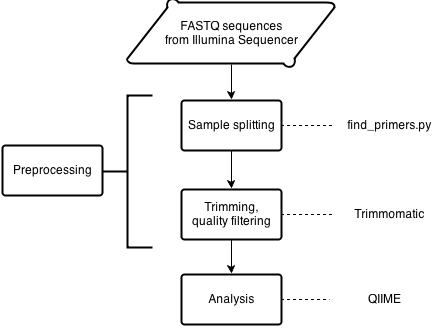
\includegraphics[width=\textwidth]{Pipeline}
		\caption{16S pipeline stages}
		\label{fig:pipeline}
	\end{figure}
	
	Every stage within a pipeline consumes a set of input files and produces a set 
	of output files, so a single run of an experiment through the pipeline will produce
	a large number of work products, which must be managed manually by the user of 
	the pipeline. \Cref{tab:stages_files} shows the number of files that will
	accumulate through running through the stages in a pipeline, which must be managed
	by the user.
	
	\begin{table}[h!]
		\centering
		\begin{tabular}{ccc}
		\toprule
		Stage & {\# of Input Files} & {\# of Output Files}\\
		\midrule
		Trimmomatic & 2 & 5 \\
		Bowtie2 & 3 & 7\\
		QIIME (Assign multiplex reads) & 3 & 3\\
		\bottomrule
		\end{tabular}
		\caption{Number of files involved in 16S pipeline stages}
		\label{tab:stages_files}
	\end{table}
	
	PIPPING was developed as an extension to PIP\cite{Conery:2005:RWM:1089844.1089845} (\emph{P}ipeline \emph{I}nterface \emph{P}rogram), a prototype 
	tool that manages bioinformatics pipelines using MySQL databases. 
	The project focused on the preprocessing (primer splitting, trimming, quality filtering) 
	stages of the pipeline, preparing the work products from the raw sequencing 
	data produced by the Illumina NGS machines to be fed into the analysis (clustering, alignment, phylogenic inference) 
	stages. Instead of using MySQL databases, PIPPING explored the feasibility of 
	storing work products in a SQLite database, with the following goals:
	
	\subsection{Reduction in intermediate work products} % (fold)
	\label{sub:reduction_in_intermediate_work_products}
	Every stage in a 16S pipeline require a set of input and output files, which increases 
	the organizational workload for the user running the pipeline. By feeding inputs and
	consuming outputs of stages, a PIPPING database can contain all data within a pipeline
	in a single file, reducing the amount of file management required of the user. 

	% subsection reduction_in_intermediate_work_products (end)

	\subsection{Reduction in overall disk usage} % (fold)
	\label{sub:reduction_in_overall_disk_usage}
	Reducing the number of intermediate work products in a pipeline also serves to reduce 
	the amount of disk space consumed by running a pipeline. Temporary work products 
	produced by converting between one file format to another can be reduced or eliminated 
	by performing data transformations in PIPPING and feeding the output to the next stage 
	directly. 

	% subsection reduction_in_overall_disk_usage (end)

	\subsection{Faster pipeline runs} % (fold)
	\label{sub:faster_pipeline_runs}
	For programs such as Trimmomatic (which requires only one pass over input data) there
	is a minor increase in processing speed due to reduced disk access. Additionally, since
	format conversions can be performed on-the-fly without disk access, conversion stages
	within a pipeline can be skipped, reducing the overall number of stages in a pipeline.
	% subsection speedup_in_runtimes (end)

	\subsection{Improving reproducibility} % (fold)
	\label{sub:improving_reproducibility}
	A PIPPING database is a container that holds not just the original sequences from the 
	Illumina Sequencer, but also results of transformations performed by stages in 
	the pipeline, and the parameters used in those transformations. Since OTU clustering 
	strategies are sensitive to length and quality filtering parameters upstream, preserving settings 
	used in earlier stages can aid analysis in later stages.
	% subsection improving_reproducibility (end)

	\subsection{Easier organization and collaboration} % (fold)
	\label{sub:easier_organization_and_collaboration}
	With all the data on an experiment contained in a single file, users can easily 
	share PIPPING databases with collaborators without needing to manage dozens of files 
	for every experiment. The semantic structure of the SQLite tables inside the database
	provide an open platform for developers to extend Pip, such as streaming adapters 
	for currently unsupported programs.
	% subsection easier_organization_and_sharing (end)
	
	%PIPPING eliminates the accumulation of intermediate work products in a pipeline by
	%containing the data within a single file (PIPPING database). It reduces the amount 
	%of disk space usage through compression and storage of logical differences between
	%the input and output of stages. By transferring only the required data to the 
	%stages in the pipeline, PIPPING reduces disk access and provides minor speedups to 
	%runtimes.
	
	% section introduction (end)
	\section{Data Management} % (fold)
	\label{sec:data_management}
	Management of data in a pipeline is conceptually divided into four tasks: 
	creating semantic structure within the database; storing sequence data in compressed form;
	transforming stored data into formats required by tools in the pipeline; logging
	settings and parameters of transformations and related metadata.
	
	As the first stage in a 16S pipeline, PIPPING combines primer sequences, barcodes, 
	offsets, and raw Illumina NGS (Next-Gen Sequencing) FASTQ files into a single, 
	compressed file that acts as a logical container for the experiment. PIPPING 
	encapsulates the data with adapters to transform the compressed data into 
	usable input for subsequent stages, and provides metadata logging. Typically, 
	an Illumina NGS machine uses \emph{Paired-End Sequencing}\cite{paired-end} to produce a pair of FASTQ files
	in the following format:

	\singlespacing
	\begin{verbatim}
@HWI-ST0747:277:D1M96ACXX:6:1101:1232:2090 1:N:0:
GGATAGTACTAGGGTATCTAATCCTGTTTGCTCCCCACGCT...
+
ACCCFFDDFH#FHHIGIJJFJJJJJJJJJJJIIJJJGIJJG...
	\end{verbatim}
	\doublespacing
	where line 1 is the \emph{defline} containing information about the Illumina
	Sequencer which produced the sequence, line 2 contains all the bases in the 
	sequence, line 3 is the separator between the sequence and quality scores, and 
	line 4 contains the corresponding quality score for each of the bases in the 
	sequence. Each character in the file ias an ASCII character taking up 8 bits. 
	The format uses five characters to represent the four DNA-bases (A - adenine, T - thymine,
	C - cytosine, G - guanine) and N to represent an errorneous read. Each base is paired
	with a quality score that has 42 values (0 to 41).

	\subsection{Semantic Database Structure} % (fold)
	\label{sub:semantic_database_structure}
	Instead of juggling multiple input files such as raw Illumina FASTQ sequences,
	barcodes, and offsets, PIPPING creates several SQLite tables which impart a well-defined
	semantic structure to the data and contains them within a single file.
	
	\begin{figure}[h!]
		\centering
		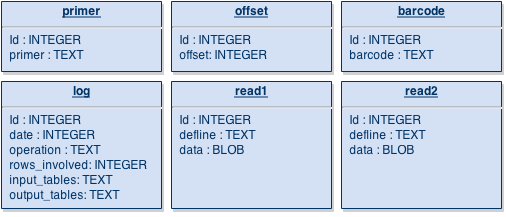
\includegraphics[width=\textwidth]{db_structure}
		\caption{PIPPING database structure}
		\label{fig:db_structure}
	\end{figure}
	\Cref{fig:db_structure} shows the structure of a PIPPING database, 
	initialized with six tables:
	
	\begin{description}
		\item[primer] holds all primer sequences used in the experiment
		\item[offset] randomized offsets to aid 16S sequencing
		\item[barcode] experiment identifier
		\item[log] stores all metadata related to data, experiment, or pipeline
		\item[read1] stores the first part of paired-end sequence data
		\item[read2] stores the second part of paired-end sequence data
	\end{description}
	
	The \emph{primer}, \emph{offset}, and \emph{barcode} tables links information 
	about the experiment to the actual sequences to be stored in the \emph{read1} 
	and \emph{read2} tables. Each sequence in the FASTQ input is stored as a row in 
	the read tables, with the bases and quality scores compressed into a binary BLOB.
	
	The \emph{log} table stores metadata about every 
	operation done in Pip. The settings used in the operation, along with the time and sequences affected
	are stored in the \emph{log} table. Since the results of OTU Analysis can be 
	affected by parameters used by the stages upstream in a pipeline, having a 
	reliable record of operations and transformations to the data will aid in 
	analysis stages downstream.
	
	Sequence data stored in \emph{read1} and \emph{read2} tables in the database are fed as input 
	to later stages in the pipeline. Correspondingly, output from those stages are 
	normalized into new tables in the database. For example, running Trimmomatic with 
	PIPPING \emph{trimmed1} and \emph{trimmed2} tables which stores the coordinates 
	of trimmed bases from the results of trimming and filtering operations performed by Trimmomatic. 
	This prevents unnecessary data duplication and reduces the file size of a PIPPING 
	database.

	% subsection database_structure (end)

	\subsection{Data Compression} % (fold)
	\label{sub:data_compression}
	Compression works by representing
	each base with an integer range (A: 0 to 49, T: 50-99, C: 100-149, G: 150-199, N: 200-255)
	and adding the quality score to the beginning of that range. Thus, base `A' with a 
	quality score of `\#' (value 0) can be represented by the value 0, while base `G' with
	a quality score of `J' (value 41) can be represented by 191 (150 + 41). The resulting
	values fit within an 8-bit character, which is a 50\% reduction in space usage. 
	Since both compression and decompression require only addition operators, the scheme
	is fast and lossless. However, the overall size of a PIPPING file is not 50\% smaller 
	than a raw FASTQ file due to the overhead involved in maintaining a valid SQLite 
	database.

	% subsection compression (end)
	
	\subsection{Data Transformation \& Flow} % (fold)
	\label{sec:data_transformation}
	A central part of managing the sequence data in the 16S pipeline is the manipulation
	and transferring of sequences between the various tools. There is often a need
	to modify the structure or format of the data to fit the varying input requirements
	of those tools. \Cref{tab:expected_input} shows the various input formats that
	tools in the pipeline require.

	\begin{table}
		\centering
		\begin{tabular}{cc}
		\toprule
		Tool & Expected input format\\
		\midrule
		Trimmomatic & FASTQ/Gzipped FASTQ\\
		Bowtie2 & FASTQ/FASTA\\
		QIIME & 454-FASTA/454-Quality Scores\\
		\bottomrule
		\end{tabular}
		\caption{Expected input formats for various tools}
		\label{tab:expected_input}
	\end{table}
 % NEED TO REPHRASE OUT VARIOUS
	Traditionally, the way to manage data in the pipeline was to store distinct sets of input 
	and output files for every stage. For example, the first stage of 
	the pipeline usually involves using Trimmomatic to filter poor quality reads 
	and to trim all the reads to a certain length. Doing this requires the user to
	provide 2 paired-end FASTQ sequence files to Trimmomatic, which will then produce
	5 output files: unpaired and paired sequences 1 and 2, and a trimming log. The 
	output files have sizes similar to the input, which results in the space usage
	nearly doubling after the first stage in the pipeline. Subsequent stages will
	then take the output of the first stage and create more output. Thus, both
	the number of files and their file size will increase very quickly due to the 
	number of stages within the 16S pipeline. Additionally, certain stages in a pipeline only exist to convert sequences from 
	one format to another (i.e.\ the need to convert Illumina FASTQ to 454-FASTA and 
	454-Quality formats required by QIIME), increasing the length of the pipeline 
	and the number of intermediate work products.
	
	Using a plug-in architecture, PIPPING can ``stream'' sequence data to tools in the
	pipeline without writing to disk. PIPPING uses UNIX Named Pipes to feed data to 
	external programs such as Trimmomatic and Bowtie2 while simultaneously consuming 
	the output they produce back into the database. UNIX Named Pipes allows programs to transfer
	data through memory instead of disk, and therefore do not require reading and
	writing to disk. However, named pipes appear as size zero, regular files on a filesystem,
	thus tools can read and write from those files without needing any changes
	to the software. In the case of Trimmomatic, PIPPING provides a named pipe to capture
	the contents of the trimming log, and uses the details within it (sequence number, 
	position of trim, number of characters trimmed) and stores them in a ``trimmed''
	table. Since this table only stores the sequences which were operated on, instead 
	of entire copies of the original sequences, the size increase of the PIPPING database
	after the first stage is almost negligible. Additionally, instead of needing to
	manage multiple output files and their naming, the data is now ready for the 
	next stage of the pipeline.
	% subsection data_flow_using_unix_pipes (end)
	% section data_management (end)

\section{Results} % (fold)
\label{sec:results}
PIPPING was benchmarked on a 2.7 GHz Intel Core i7 processor with 16GB of RAM, running
OS X 10.9. \Cref{tab:insertion_speeds} shows the time taken for the specified number
of sequence inserts into a new PIPPING database. \Cref{fig:insertion_speeds} plots the
number of actual raw inserts per second into SQLite, showing consistent insertion 
rates between \np{96000} and \np{102000} raw inserts per second.

\begin{table}[h!]
\centering
\begin{tabular}{n{4}{2}n{4}{2}}
	\toprule
 {Number of sequences (paired-end)} & {Time taken (seconds)} \\
 \midrule
 \np{500000} & 10.35 \\
 \np{1000000} & 19.57 \\
 \np{2000000} & 39.22 \\
 \np{4000000} & 78.67 \\
 \np{8000000} & 160.84 \\
 \np{16000000} & 319.38 \\
 \np{32000000} & 644.90 \\
 \np{64000000} & 1286.26 \\
 \bottomrule
\end{tabular}
\caption{Insertion speeds into SQLite using Pip}
\label{tab:insertion_speeds}
\end{table}

\begin{figure}[h!]
	\centering
	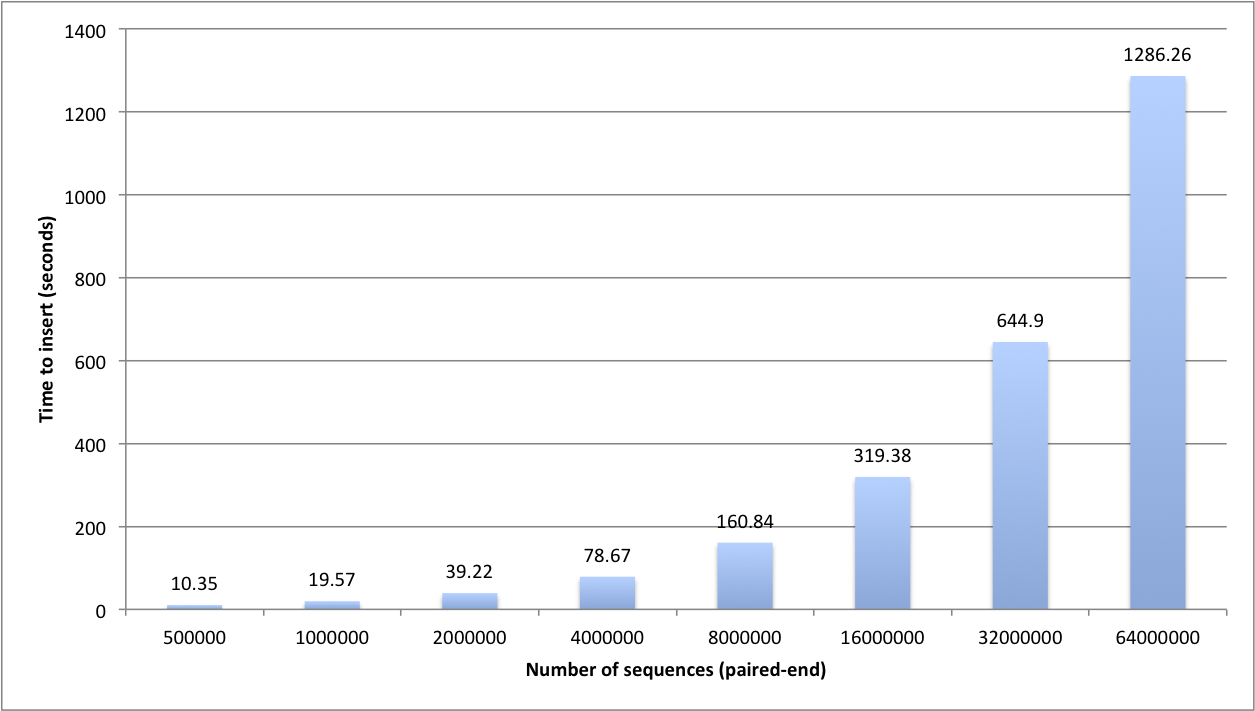
\includegraphics[width=\textwidth]{insertion_speed_chart}
	\caption{Inserts per second into SQLite using PIPPING}
	\label{fig:insertion_speeds}
\end{figure}
\newpage
\Cref{tab:filesizes} shows the size of the raw FASTQ sequence file compared to the resulting
database file after inserts. \Cref{fig:filesizes} reveals a consistent
45\% reduction in file size after insertions.

\begin{table}[h!]
\centering
\begin{tabular}{n{0}{0}n{6}{2}n{6}{2}}
	\toprule
 {Number of sequences (paired-end)} & {Input FASTQ size (MB)} & {PIPPING database (MB)} \\
 \midrule
 \np{500000} & 371.40 & 206.90 \\
 \np{1000000} & 743.00 & 413.90 \\
 \np{2000000} & 1486.00 & 828.00 \\
 \np{4000000} & 3051.52 & 1699.84 \\
 \np{8000000} & 6082.56 & 3389.44 \\
 \np{16000000} & 12165.12 & 6789.12 \\
 \np{32000000} & 24350.72 & 13568.00 \\
 \np{64000000} & 48701.44 & 27146.20 \\
 \np{91000000} & 69754.88 & 35061.76 \\
 \bottomrule
\end{tabular}
\caption{Comparison of input file sizes against PIPPING database sizes}
\label{tab:filesizes}
\end{table}

\begin{figure}[h!]
	\centering
	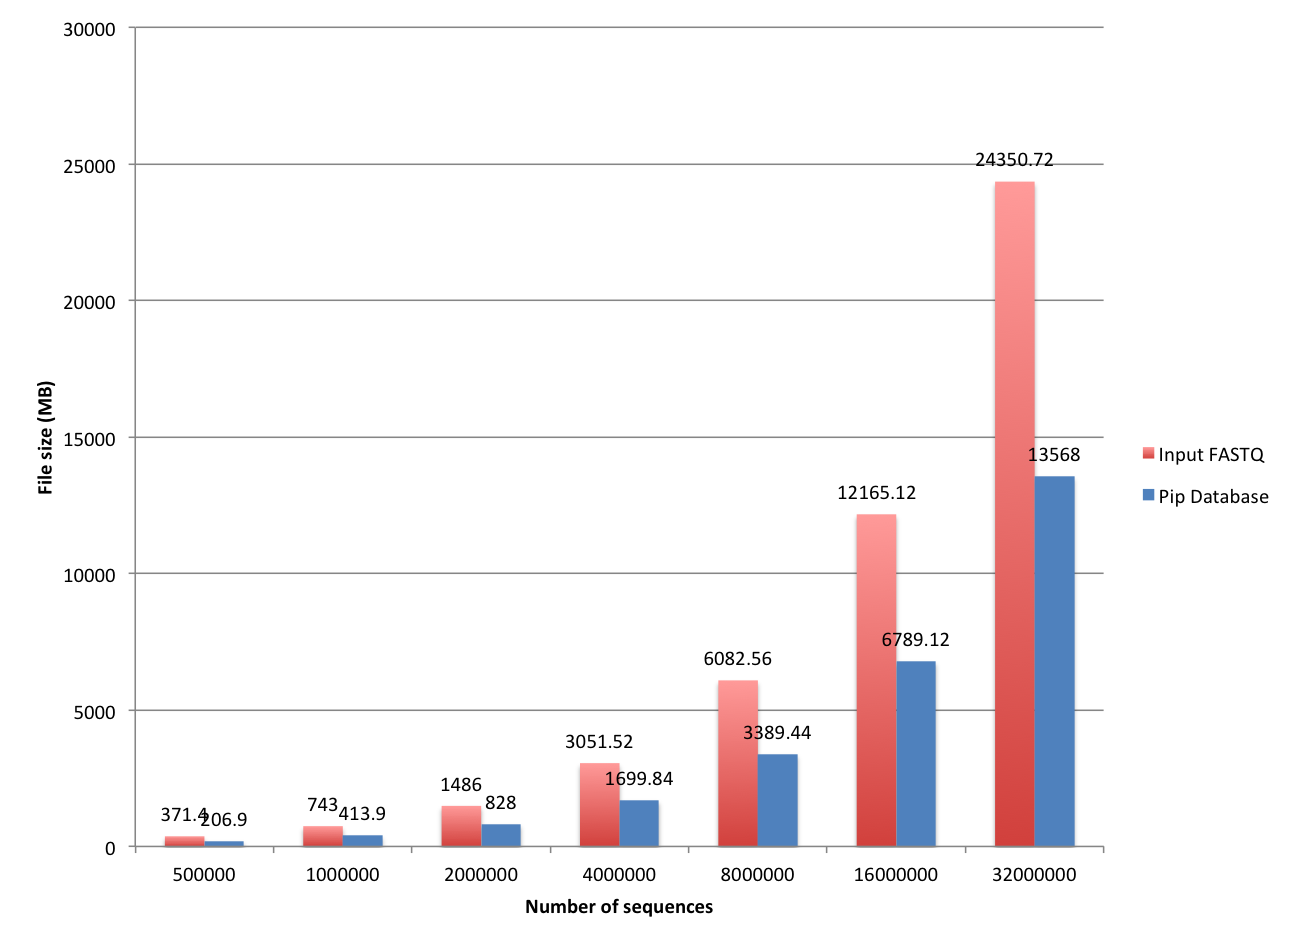
\includegraphics[width=\textwidth]{filesizes_chart}
	\caption{File sizes of PIPPING database against original FASTQ files}
	\label{fig:filesizes}
\end{figure}

\Cref{tab:streamspeed} shows runtime reductions in a stage in the test pipeline, 
as a result of streaming data directly from PIPPING to Trimmomatic, instead of accessing
the disk.

\begin{table}[h!]
\centering
\begin{tabular}{cn{6}{2}n{6}{2}}
	\toprule
 {Pipeline Stage} & {Raw time (seconds)} & {PIPPING time (seconds)} \\
 \midrule
 Trimmomatic & 46.43 & 22.89 \\
 \bottomrule
\end{tabular}
\caption{Time needed to process \np{500000} sequences through 16S pipeline stages with and without PIPPING}
\label{tab:streamspeed}
\end{table}

% section results (end)

\section{Conclusion} % (fold)
\label{sec:conclusion}
The use of PIPPING within the 16S pipeline shows promise in reducing the logistical
effort of researcher and interoperability headaches of multiple tools. PIPPING currently 
operates on the preprocessing stages of a 16S pipeline and can be extended to later
stages in the pipeline easily through a plug-in architecture. The number of intermediate 
work products in a pipeline has been reduced to a single PIPPING database file, and there 
are measurable reductions in pipeline run times. There appears to be 
negligible overhead in streaming data compared to transferring data over the filesystem 
using intermediate files, and the underlying SQLite implementation is able to
deal with datasets of almost 100 million rows without slowdowns. The plug-in architecture
of PIPPING can be extended in the future to support other pipelines such as UPARSE\cite{uparse} or
QIIME\cite{qiime}.

However, PIPPING currently does not perform complex queries such as subtable queries in 
its current pipeline so we do not have data on possible scalability issues. SQLite itself
might also be a limiting factor due to its single-access model\cite{sqlitewhen}, so it might not work
well for distributed or parallel workflow projects such as PaPy\cite{21352538} or
Parallel-META\cite{23046922}.
% section conclusion (end)

\bibliographystyle{plain}
\bibliography{citations}
\end{document}
